\begin{frame}{Circuito de interconexión}
			\centering
			\rowcolors{2}{black!15}{white}
%	\begin{itemize}
%		\only<1>{
%			\item Versión 1\\
%			\centering
%			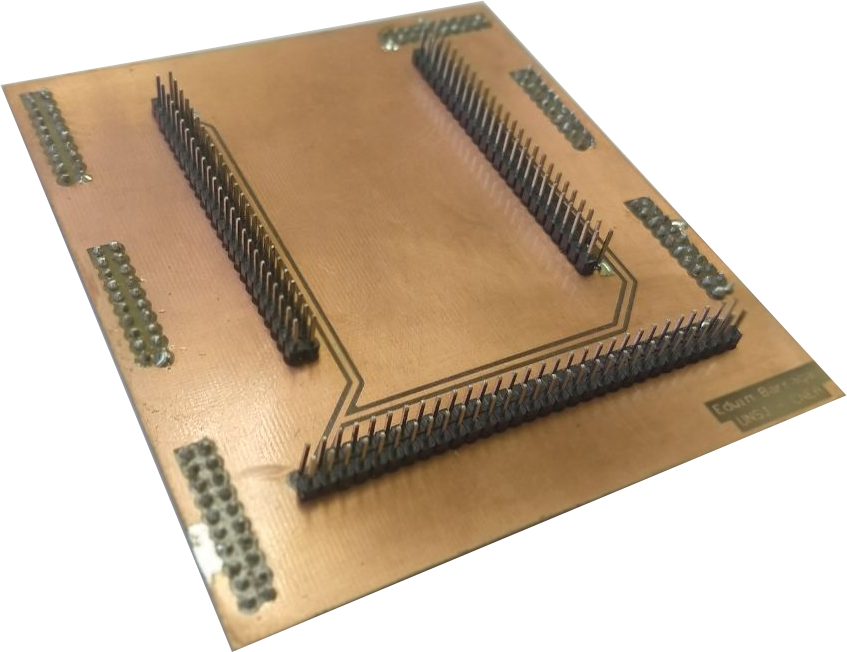
\includegraphics[width=.45\textwidth]{61v1anverso}
%			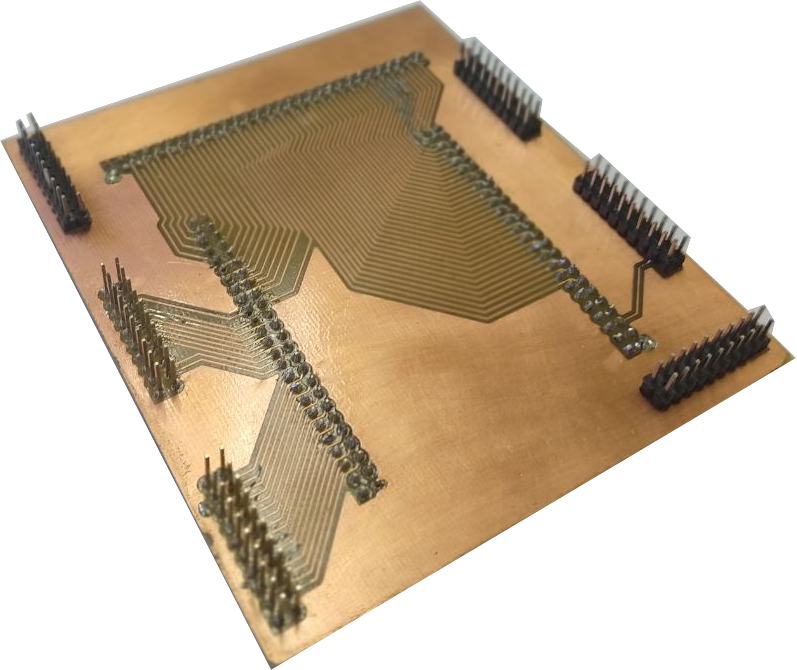
\includegraphics[width=.45\textwidth]{62v1reverso}
%		}			
		\only<1>{
%			\item Versión 2\\
			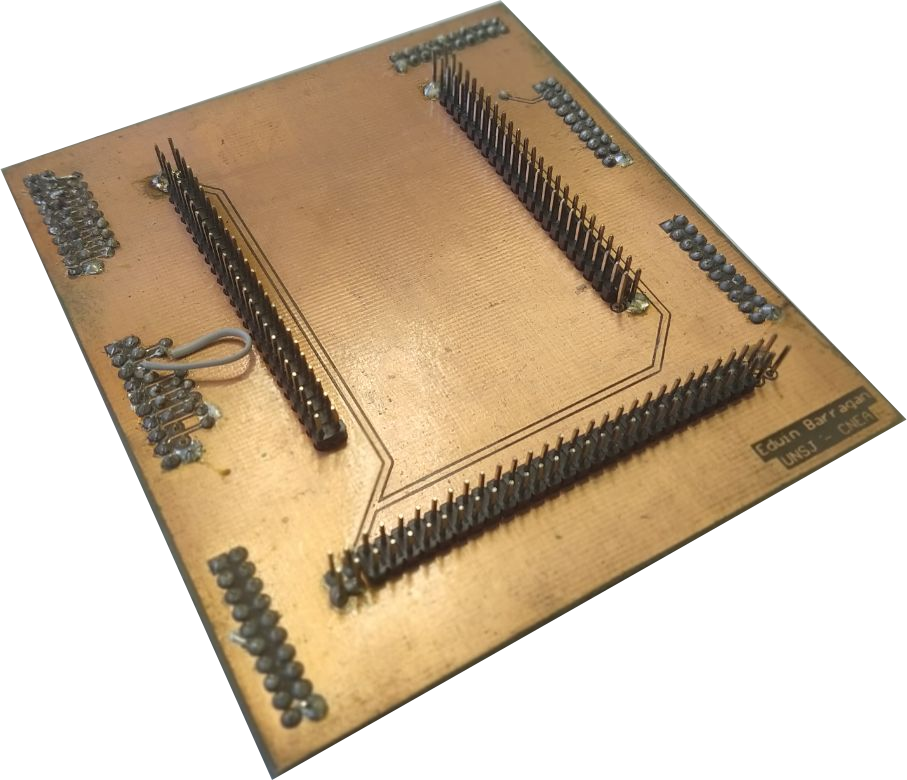
\includegraphics[width=.45\textwidth]{63v2anverso}
			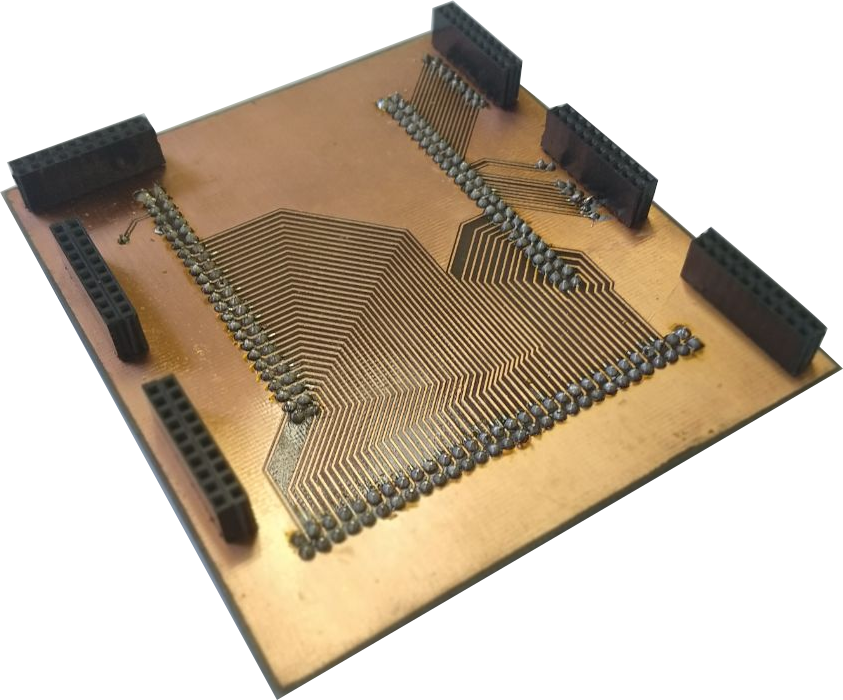
\includegraphics[width=.45\textwidth]{64v2reverso}
		}
		\only<2>{
%			\item Versión 3\\
%			\centering
			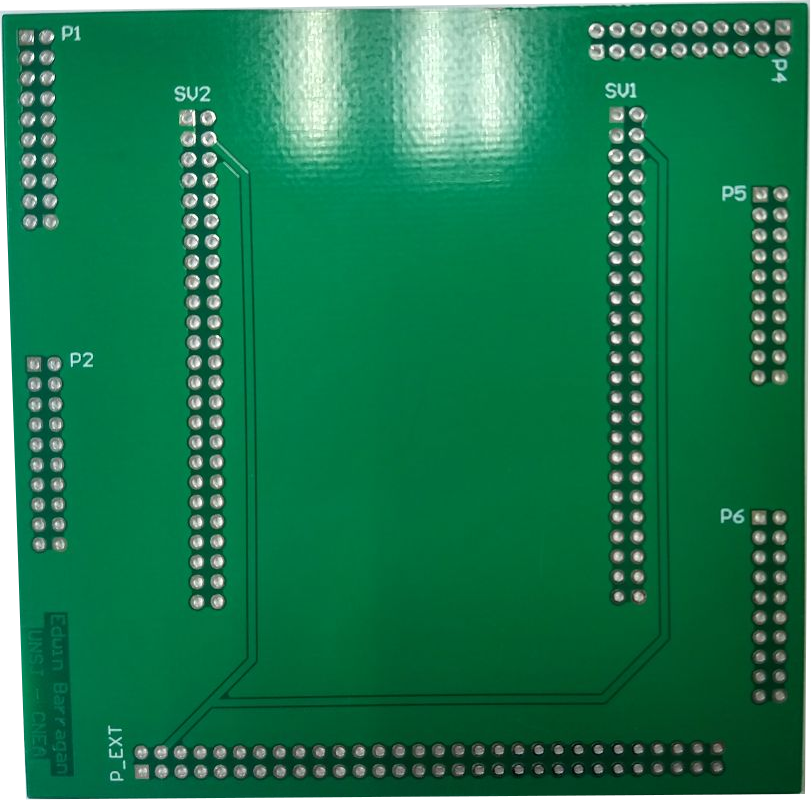
\includegraphics[width=.45\textwidth]{65v3anverso}
			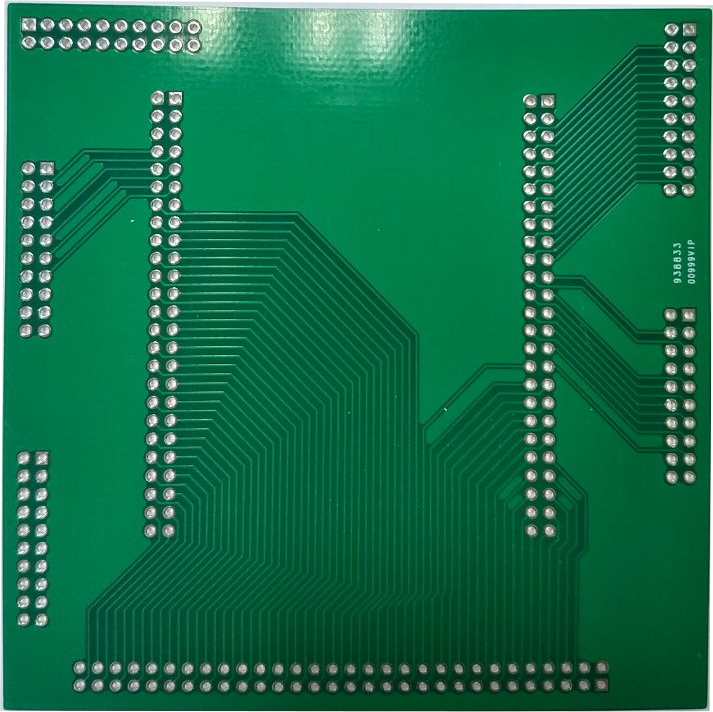
\includegraphics[width=.45\textwidth]{66v3reverso}
		}
		\only<3>{
			\begin{tabular}{lr|lr}
%				\hline
				\textbf{FX2LP} & \textbf{Spartan 6}&\textbf{FX2LP} & \textbf{Spartan 6} \\\hline
				FD15 & P50 &FD2 & P24\\
				FD14 & P51 &FD1 & P21\\
				FD13 & P40 &FD0 & P22\\
				FD12 & P41 &SLWR & P17\\
				FD11 & P34 &SLRD & P16\\
				FD10 & P35 &SLOE & P6\\
				FD9 & P32 &FLAGA & P12\\
				FD8 & P33 &FLAGB & P14\\
				FD7 & P29 &FLAGC & P15\\
				FD6 & P30 &FLAGD & P11\\
				FD5 & P26 &PKTEND & P10\\
				FD4 & P27 &FIFOADR1 & P9\\
				FD3 & P23 &FIFOADR0 & P8\\
%				\hline
			\end{tabular}
		}
%	\end{itemize}
\end{frame}
\begin{frame}{Sistema completo}
	\centering
	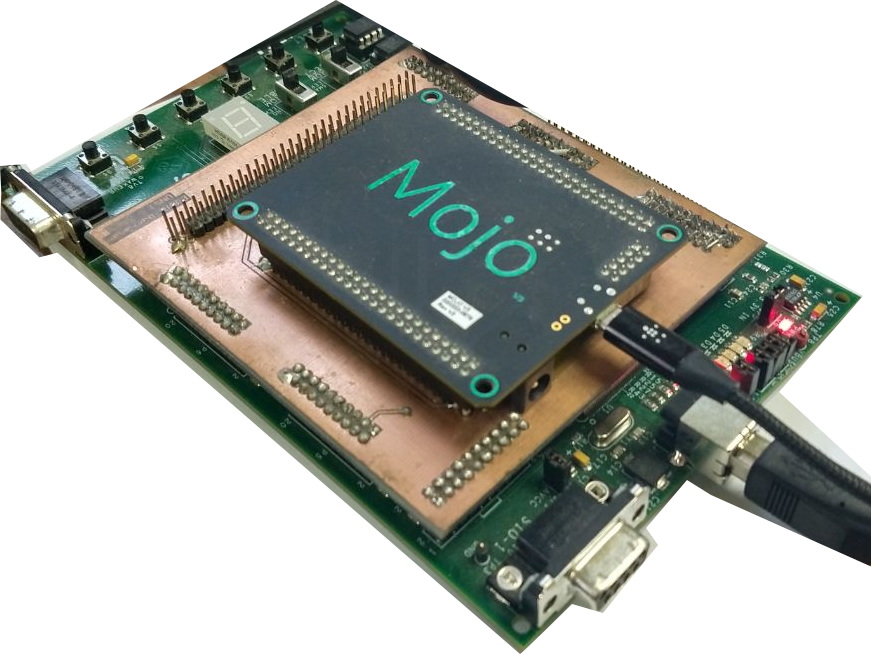
\includegraphics[width=.6\textwidth]{fisico}
\end{frame}
